% Options for packages loaded elsewhere
% Options for packages loaded elsewhere
\PassOptionsToPackage{unicode}{hyperref}
\PassOptionsToPackage{hyphens}{url}
\PassOptionsToPackage{dvipsnames,svgnames,x11names}{xcolor}
%
\documentclass[
  letterpaper,
  DIV=11,
  numbers=noendperiod]{scrartcl}
\usepackage{xcolor}
\usepackage{amsmath,amssymb}
\setcounter{secnumdepth}{-\maxdimen} % remove section numbering
\usepackage{iftex}
\ifPDFTeX
  \usepackage[T1]{fontenc}
  \usepackage[utf8]{inputenc}
  \usepackage{textcomp} % provide euro and other symbols
\else % if luatex or xetex
  \usepackage{unicode-math} % this also loads fontspec
  \defaultfontfeatures{Scale=MatchLowercase}
  \defaultfontfeatures[\rmfamily]{Ligatures=TeX,Scale=1}
\fi
\usepackage{lmodern}
\ifPDFTeX\else
  % xetex/luatex font selection
\fi
% Use upquote if available, for straight quotes in verbatim environments
\IfFileExists{upquote.sty}{\usepackage{upquote}}{}
\IfFileExists{microtype.sty}{% use microtype if available
  \usepackage[]{microtype}
  \UseMicrotypeSet[protrusion]{basicmath} % disable protrusion for tt fonts
}{}
\makeatletter
\@ifundefined{KOMAClassName}{% if non-KOMA class
  \IfFileExists{parskip.sty}{%
    \usepackage{parskip}
  }{% else
    \setlength{\parindent}{0pt}
    \setlength{\parskip}{6pt plus 2pt minus 1pt}}
}{% if KOMA class
  \KOMAoptions{parskip=half}}
\makeatother
% Make \paragraph and \subparagraph free-standing
\makeatletter
\ifx\paragraph\undefined\else
  \let\oldparagraph\paragraph
  \renewcommand{\paragraph}{
    \@ifstar
      \xxxParagraphStar
      \xxxParagraphNoStar
  }
  \newcommand{\xxxParagraphStar}[1]{\oldparagraph*{#1}\mbox{}}
  \newcommand{\xxxParagraphNoStar}[1]{\oldparagraph{#1}\mbox{}}
\fi
\ifx\subparagraph\undefined\else
  \let\oldsubparagraph\subparagraph
  \renewcommand{\subparagraph}{
    \@ifstar
      \xxxSubParagraphStar
      \xxxSubParagraphNoStar
  }
  \newcommand{\xxxSubParagraphStar}[1]{\oldsubparagraph*{#1}\mbox{}}
  \newcommand{\xxxSubParagraphNoStar}[1]{\oldsubparagraph{#1}\mbox{}}
\fi
\makeatother


\usepackage{longtable,booktabs,array}
\usepackage{calc} % for calculating minipage widths
% Correct order of tables after \paragraph or \subparagraph
\usepackage{etoolbox}
\makeatletter
\patchcmd\longtable{\par}{\if@noskipsec\mbox{}\fi\par}{}{}
\makeatother
% Allow footnotes in longtable head/foot
\IfFileExists{footnotehyper.sty}{\usepackage{footnotehyper}}{\usepackage{footnote}}
\makesavenoteenv{longtable}
\usepackage{graphicx}
\makeatletter
\newsavebox\pandoc@box
\newcommand*\pandocbounded[1]{% scales image to fit in text height/width
  \sbox\pandoc@box{#1}%
  \Gscale@div\@tempa{\textheight}{\dimexpr\ht\pandoc@box+\dp\pandoc@box\relax}%
  \Gscale@div\@tempb{\linewidth}{\wd\pandoc@box}%
  \ifdim\@tempb\p@<\@tempa\p@\let\@tempa\@tempb\fi% select the smaller of both
  \ifdim\@tempa\p@<\p@\scalebox{\@tempa}{\usebox\pandoc@box}%
  \else\usebox{\pandoc@box}%
  \fi%
}
% Set default figure placement to htbp
\def\fps@figure{htbp}
\makeatother





\setlength{\emergencystretch}{3em} % prevent overfull lines

\providecommand{\tightlist}{%
  \setlength{\itemsep}{0pt}\setlength{\parskip}{0pt}}



 


\KOMAoption{captions}{tableheading}
\makeatletter
\@ifpackageloaded{tcolorbox}{}{\usepackage[skins,breakable]{tcolorbox}}
\@ifpackageloaded{fontawesome5}{}{\usepackage{fontawesome5}}
\definecolor{quarto-callout-color}{HTML}{909090}
\definecolor{quarto-callout-note-color}{HTML}{0758E5}
\definecolor{quarto-callout-important-color}{HTML}{CC1914}
\definecolor{quarto-callout-warning-color}{HTML}{EB9113}
\definecolor{quarto-callout-tip-color}{HTML}{00A047}
\definecolor{quarto-callout-caution-color}{HTML}{FC5300}
\definecolor{quarto-callout-color-frame}{HTML}{acacac}
\definecolor{quarto-callout-note-color-frame}{HTML}{4582ec}
\definecolor{quarto-callout-important-color-frame}{HTML}{d9534f}
\definecolor{quarto-callout-warning-color-frame}{HTML}{f0ad4e}
\definecolor{quarto-callout-tip-color-frame}{HTML}{02b875}
\definecolor{quarto-callout-caution-color-frame}{HTML}{fd7e14}
\makeatother
\makeatletter
\@ifpackageloaded{caption}{}{\usepackage{caption}}
\AtBeginDocument{%
\ifdefined\contentsname
  \renewcommand*\contentsname{Table of contents}
\else
  \newcommand\contentsname{Table of contents}
\fi
\ifdefined\listfigurename
  \renewcommand*\listfigurename{List of Figures}
\else
  \newcommand\listfigurename{List of Figures}
\fi
\ifdefined\listtablename
  \renewcommand*\listtablename{List of Tables}
\else
  \newcommand\listtablename{List of Tables}
\fi
\ifdefined\figurename
  \renewcommand*\figurename{Figure}
\else
  \newcommand\figurename{Figure}
\fi
\ifdefined\tablename
  \renewcommand*\tablename{Table}
\else
  \newcommand\tablename{Table}
\fi
}
\@ifpackageloaded{float}{}{\usepackage{float}}
\floatstyle{ruled}
\@ifundefined{c@chapter}{\newfloat{codelisting}{h}{lop}}{\newfloat{codelisting}{h}{lop}[chapter]}
\floatname{codelisting}{Listing}
\newcommand*\listoflistings{\listof{codelisting}{List of Listings}}
\makeatother
\makeatletter
\makeatother
\makeatletter
\@ifpackageloaded{caption}{}{\usepackage{caption}}
\@ifpackageloaded{subcaption}{}{\usepackage{subcaption}}
\makeatother
\usepackage{bookmark}
\IfFileExists{xurl.sty}{\usepackage{xurl}}{} % add URL line breaks if available
\urlstyle{same}
\hypersetup{
  pdftitle={Decision Tree Challenge},
  colorlinks=true,
  linkcolor={blue},
  filecolor={Maroon},
  citecolor={Blue},
  urlcolor={Blue},
  pdfcreator={LaTeX via pandoc}}


\title{Decision Tree Challenge}
\usepackage{etoolbox}
\makeatletter
\providecommand{\subtitle}[1]{% add subtitle to \maketitle
  \apptocmd{\@title}{\par {\large #1 \par}}{}{}
}
\makeatother
\subtitle{Feature Importance and Categorical Variable Encoding}
\author{}
\date{}
\begin{document}
\maketitle


\section{🌳 Decision Tree Challenge - Feature Importance and Variable
Encoding}\label{decision-tree-challenge---feature-importance-and-variable-encoding}

\textbf{How does encoding categorical variables as numbers affect our
understanding of feature importance?}

For detailed analysis and conclusions, see the Discussion
Section(\#sec-Discussion).

\subsection{The Ames Housing Dataset 🏠}\label{the-ames-housing-dataset}

We are analyzing the Ames Housing dataset which contains detailed
information about residential properties sold in Ames, Iowa from 2006 to
2010. This dataset is perfect for our analysis because it contains a
categorical variable (like zip code) and numerical variables (like
square footage, year built, number of bedrooms).

\subsection{The Problem: ZipCode as Numerical vs
Categorical}\label{the-problem-zipcode-as-numerical-vs-categorical}

\textbf{Key Question:} What happens when we treat zipCode as a numerical
variable in a decision tree? How does this affect feature importance
interpretation?

\textbf{The Issue:} Zip codes (50010, 50011, 50012, 50013) are
categorical variables representing discrete geographic areas,
i.e.~neighborhoods. When treated as numerical, the tree might split on
``zipCode \textgreater{} 50012.5'' - which has no meaningful
interpretation for house prices. Zip codes are non-ordinal categorical
variables meaning they have no inherent order that aids house price
prediction (i.e.~zip code 99999 is not the priceiest zip code).

\subsection{Data Loading and Model
Building}\label{data-loading-and-model-building}

\subsubsection{R}\label{r}

\begin{verbatim}
Model built with 7 terminal nodes
\end{verbatim}

\subsection{Tree Visualization}\label{tree-visualization}

\subsubsection{R}

\pandocbounded{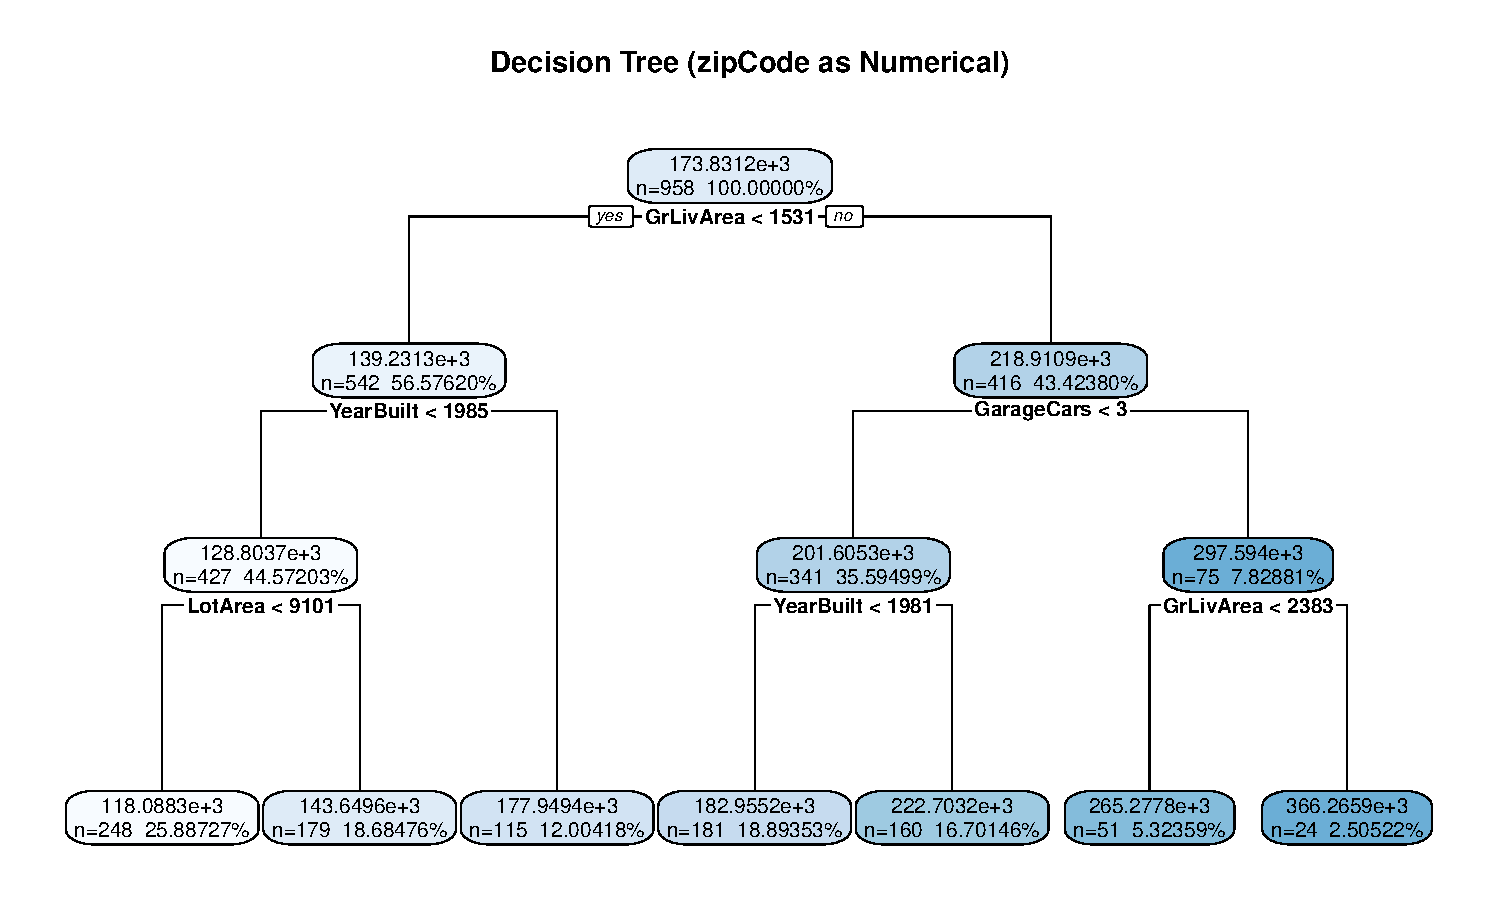
\includegraphics[keepaspectratio]{index_files/figure-pdf/visualize-tree-r-1.pdf}}

\subsection{Feature Importance
Analysis}\label{feature-importance-analysis}

\subsubsection{R}

\pandocbounded{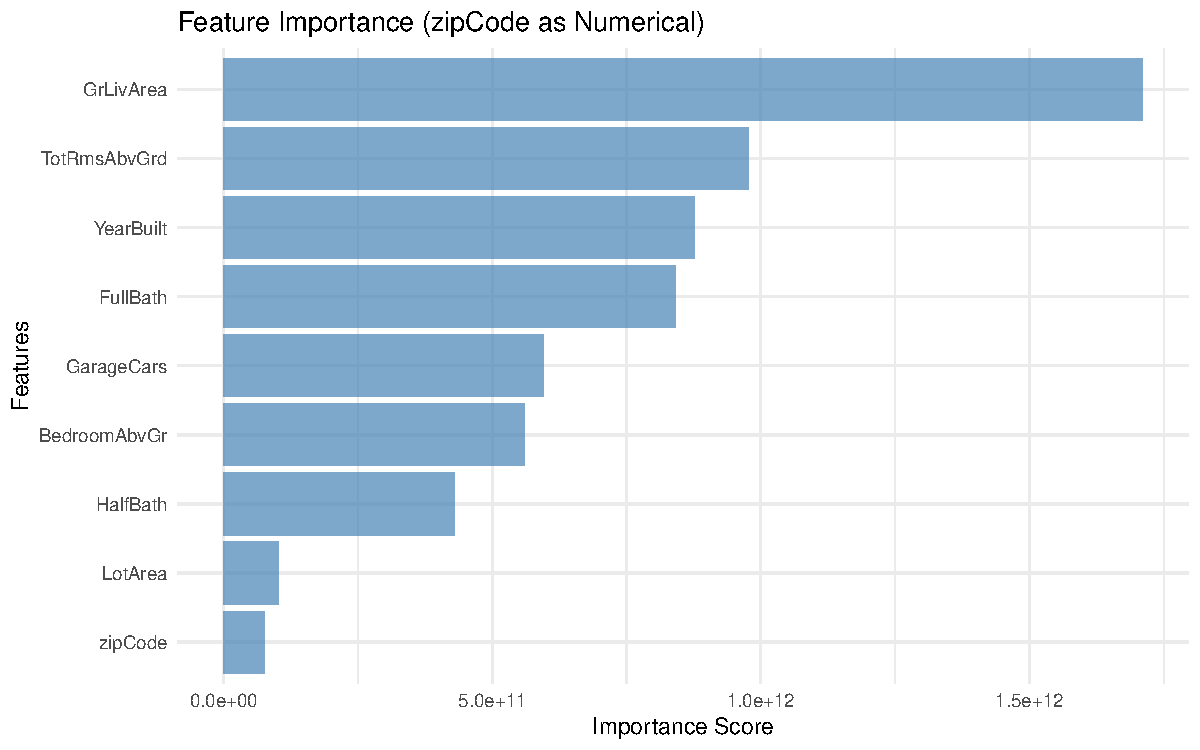
\includegraphics[keepaspectratio]{index_files/figure-pdf/importance-plot-r-1.pdf}}

\subsection{Critical Analysis: The Encoding
Problem}\label{critical-analysis-the-encoding-problem}

\begin{tcolorbox}[enhanced jigsaw, toprule=.15mm, left=2mm, breakable, colbacktitle=quarto-callout-warning-color!10!white, opacitybacktitle=0.6, coltitle=black, colback=white, colframe=quarto-callout-warning-color-frame, title=\textcolor{quarto-callout-warning-color}{\faExclamationTriangle}\hspace{0.5em}{⚠️ The Problem Revealed}, rightrule=.15mm, toptitle=1mm, titlerule=0mm, opacityback=0, bottomtitle=1mm, arc=.35mm, bottomrule=.15mm, leftrule=.75mm]

\textbf{What to note:} Our decision tree treated \texttt{zipCode} as a
numerical variable. This leads to zip code being unimportant. Not
surprisingly, because there is no reason to believe allowing splits like
``zipCode \textless{} 50012.5'' should be beneficial for house price
prediction. This false coding of a variable creates several problems:

\begin{enumerate}
\def\labelenumi{\arabic{enumi}.}
\tightlist
\item
  \textbf{Potentially Meaningless Splits:} A zip code of 50013 is not
  ``greater than'' 50012 in any meaningful way for house prices
\item
  \textbf{False Importance:} The algorithm assigns importance to zipCode
  based on numerical splits rather than categorical distinctions OR the
  importance of zip code is completely missed as numerical ordering has
  no inherent relationship to house prices.
\item
  \textbf{Misleading Interpretations:} We might conclude zipCode is not
  important when our intuition tells us it should be important (listen
  to your intuition).
\end{enumerate}

\textbf{The Real Issue:} Zip codes are categorical variables
representing discrete geographic areas. The numerical values have no
inherent order or magnitude relationship to house prices. These must be
modelled as categorical variables.

\end{tcolorbox}

\subsection{Proper Categorical Encoding: The
Solution}\label{proper-categorical-encoding-the-solution}

Now let's repeat the analysis with zipCode properly encoded as
categorical variables to see the difference.

\textbf{R Approach:} Convert zipCode to a factor (categorical variable)

\subsubsection{Categorical Encoding Analysis}

\subsubsection{R}

\subsubsection{Feature Importance: Categorical zipCode}

\subsubsection{R}

\pandocbounded{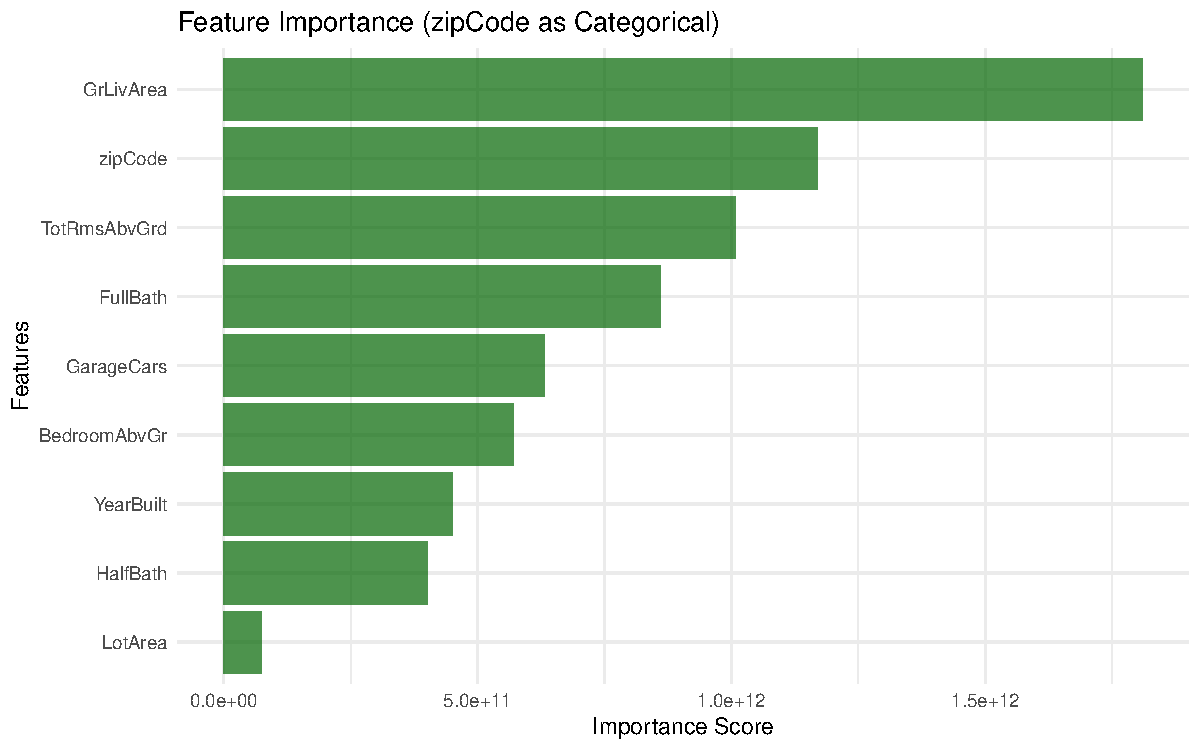
\includegraphics[keepaspectratio]{index_files/figure-pdf/importance-plot-cat-r-1.pdf}}

\subsection{Discussion}\label{discussion}

\begin{enumerate}
\def\labelenumi{\arabic{enumi}.}
\tightlist
\item
  \textbf{Numerical vs Categorical Encoding:}
\end{enumerate}

I know that there is no difference higher zip codes vs lower zip codes
which means that modeling numerically does not make much sense because
the value of the numbers within a zip codes does not tell us anything.
But, modeling categorically allows us to treat each zip code as its own
category which helps with analysis.

\begin{enumerate}
\def\labelenumi{\arabic{enumi}.}
\setcounter{enumi}{1}
\tightlist
\item
  \textbf{R vs Python Implementation Differences:}
\end{enumerate}

R does a better job when modeling a categorical variable because the
Python importance chart attempts to show the importance of each zip code
in the dataset which does not help us since there are so many. This is
because Python creates a dummy variable for each zip code while R uses a
factor to make zip codes categorical. This is why each individual zip
code shows up on the Python feature importance graph. There is some
documentation saying that the langugage Julia can handle categorical
variables effectively. Julia documentation states, ``CategoricalVector
\ldots{} is designed to additionally provide full support for working
with categorical variables, both with unordered (nominal variables) and
ordered categories (ordinal variables)'' which shows Julia's versatility
when it comes to these kinds of variables.

\begin{enumerate}
\def\labelenumi{\arabic{enumi}.}
\setcounter{enumi}{2}
\tightlist
\item
  \textbf{Professional Presentation:}
\end{enumerate}

\section{Discussion Section:}\label{discussion-section}

See \textbf{?@sec-Discussion} for a discussion of categorical variables




\end{document}
